\chapter{Introduction}
The Large Hadron Collider (LHC) is the largest particle accelerator in the world. During the first run of it from 2010 to 2013 its experiments had made remarkable achievements. Perhaps one of the most famous is the discovery of the theorised Higgs particle, which resulted in the Nobel Prize in Physics in 2013 being awarded to François Englert and Peter Higgs. The LHC are made to collide particles at four locations around the accelerator ring, corresponding to the positions of four particle detectors – ATLAS, CMS, ALICE and LHCb \cite{ref_cern_home}.


\section{Compact Muon Solenoid}

The Compact Muon Solenoid (CMS) is a cylindrical particle detector designed to measure a wide range of particles produced in the collisions of LHC. The size of the detector is around 28 m long and 15 m in diameter. It is the heaviest detector in the world and weighs approximately 14000 t. The name "CMS" originates from the three key characteristics of the detector: its relatively compact size, its excellent capabilities in the detection and measurement of muons and its central feature, a superconducting 3.8T solenoid magnet \cite{Reference1}.\\
The CMS detector consists of many separate detector layers, each of them playing an individual role in detecting and measuring the traversing particles. A cross-sectional overview of the layers and its tasks in reconstructing tracks of particles is shown in the
figure \ref{fig:cms_layers}.
\begin{figure}[ht]\centering
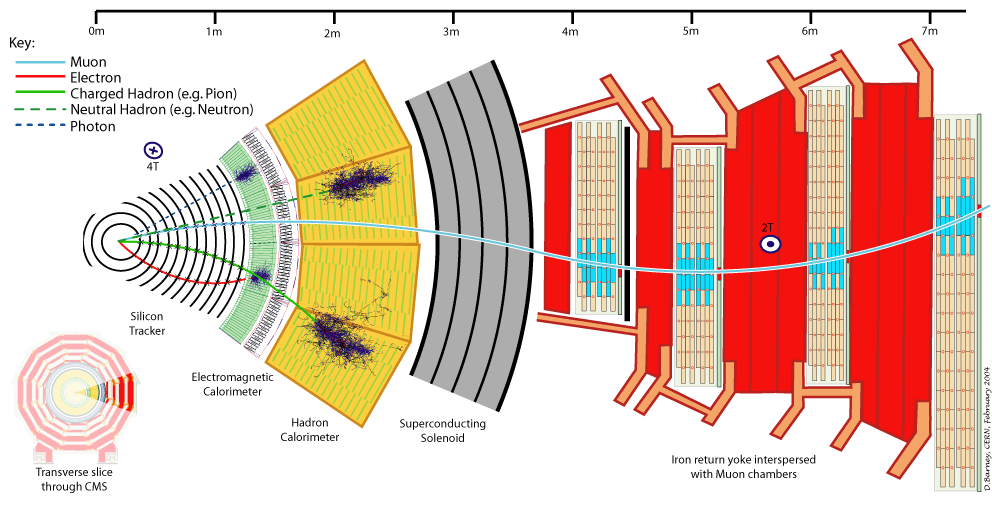
\includegraphics[width=0.8\linewidth]{Data/CMS_layers.png}
\caption{A cross-sectional view of the CMS detection layers.}
\label{fig:cms_layers}
\end{figure}

\section{Phase II Upgrade}

The CMS Phase-II Tracker will utilize two types of modules, 2S modules and PS modules. To achieve efficient rejection of low-pT particles throughout the Tracker volume, modules in different regions will make use of a few different sensor spacings. For 2S (PS) modules, spacings of 1.8 and 4 mm (1.6, 2.6 and 4 mm) are foreseen. These modules will be used in the end-cap disks as well as the central barrel region of the Tracker. An exploded view of a PS module is shown in Figure ??. In the PS module, the sensors are glued to a carbon-fibre reinforced Aluminium (AL-CF) spacers which act as spacers and provide the thermal conductance crucial for the cooling of the module. The two sensors and spacers are in turn glued the carbon-fibre (CF) baseplate. This structure is henceforth referred to as the sensor-spacer-baseplate-assembly (SSBA). This project will focus on the assembly of the SSBA only. The precision requirements of the SSBA are shown in figure ??. For the PS module, the sensors must align to within 40 mm measured at the sensor’s short edge. This corresponds to a rotational alignment tolerance of 0.8 mrad.

\subsection{Two layer Sensors}


\subsection{Assembly of two layer sensors}

